%%%%%%%%%%%%%%%%%%%%%%%%%%%%%%%%%%%%%%%%%%%%%%%%%%%%%%%%%%%%%%%%%%%%%%%%%%%%%%%%
%2345678901234567890123456789012345678901234567890123456789012345678901234567890
%        1         2         3         4         5         6         7         8
% THESIS CHAPTER

\chapter[Control Architecture: Simulation Results]{Control Architecture: \\ Simulation Results}
\label{chap:results}
\ifpdf
\graphicspath{{Results/Figures/PNG/}{Results/Figures/PDF/}{Results/Figures/}}
\else
\graphicspath{{Results/Figures/EPS/}{Results/Figures/}}
\fi

\begin{figure}[H]
	\centering
	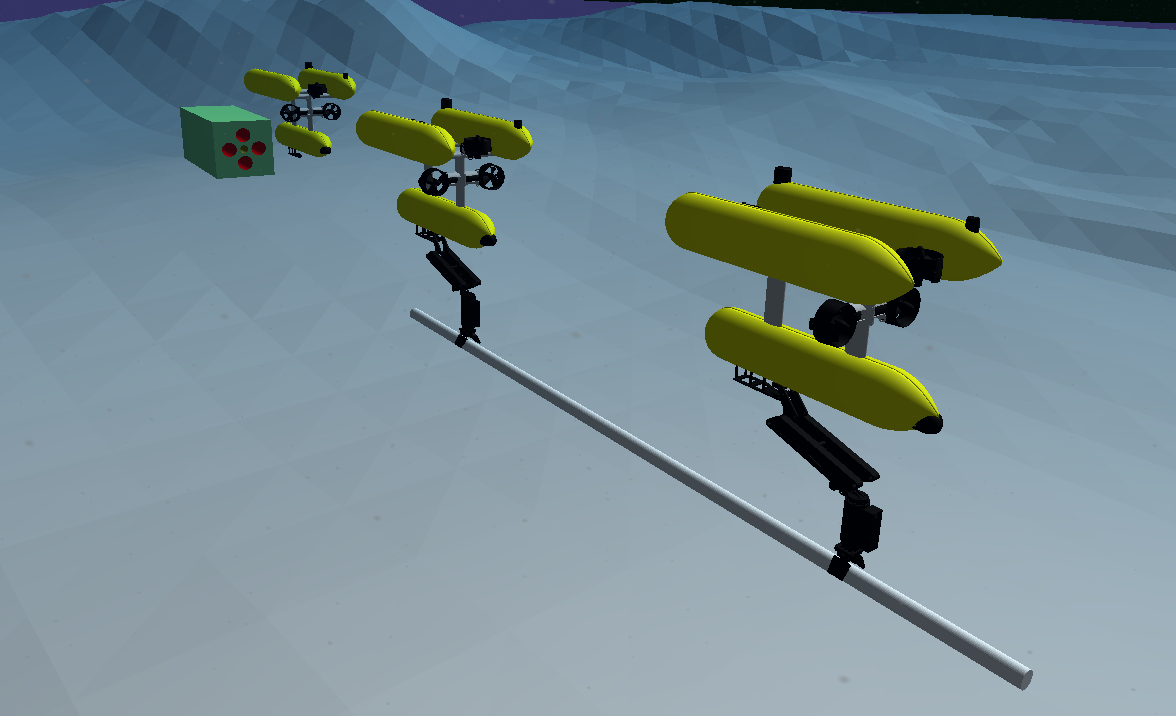
\includegraphics[width=14.5cm]{scenario_whole.png}
	\caption[The Scenario with the two robot carrying the peg and the vision robot watching the hole]{The Scenario of the experiment. The two twin robots are carrying the common peg, while the third robot is watching the hole to estimate its pose.}
	\label{fig:method_uwsim}
\end{figure}

In this chapter, experimental set-up is described, and results are given and discussed. The code for the whole architecture is available at \href{https://github.com/torydebra/AUV-Coop-Assembly}{https://github.com/torydebra/AUV-Coop-Assembly}.\\
%todo and explained a bit in the appendix?

The scenario is made up of two I-AUV's \href{https://cirs.udg.edu/auvs-technology/auvs/girona-500-auv/}{Girona 500 AUV} underwater vehicles, each one equipped with a CSIP Robot arm5E (4 DOF arm with a parallel yaw gripper). The final goal is to successfully coordinate the robots in such a way that the peg, hold by both manipulators, is inserted correctly in the hole, fixed in the environment. In the literature, this problem is known as \textit{peg-in-hole}.\\
One robot is equipped with a force torque sensor that permits to understand forces applied on the peg, caused during the insertion phase. This information is provided to both robots. A third robot estimates the hole pose in a preliminary phase. The figure \ref{fig:method_uwsim} shows what has just been described.\\
The chosen strategy divides the problem in two phases: Hole Detection and Insertion. In the first, preliminary steps are done to detect the hole. A third robot, not used for manipulation task, is in charge to exploit computer vision algorithms to estimate the pose of the hole. Detail about this are given in section \ref{chap:vision}.
The second phase explores the problems inherent to transportation of the tool, the interaction between the peg and the hole, and the communication between the carrying agents. This is described in this chapter.

\section{Choosing the Simulator}
\label{sec:simulators}
A bit effort has been spent to choice a suitable simulator for the case. At the end, \href{http://www.irs.uji.es/uwsim/}{UWSim} [\cite{uwsim}] was chosen. It is a simulator largely used for this kind of scenarios, which visualize a virtual underwater scene. It provides a different variety of useful sensors (e.g. the used force-torque sensor and the cameras), but also others can be added. It is fully integrate in ROS, which made it really easy to use. ROS is used as simulator interface: through ROS messages, we can send commands to the robots and we can receive information from the going on test. Contact physics is implemented integrating the physics engine \href{https://pybullet.org/wordpress/}{Bullet} with \href{http://www.openscenegraph.org/}{OSG} through \href{https://github.com/mccdo/osgbullet}{OSGBullet}. To further details about how the simulation is implemented, especially the contact physics part, please refers to the documentation of the cited software. The cons in using UWSim is that the simulations is fully kinematic, so no dynamics interaction ar present. This means, for example, that velocity sent to the robot are immediately accomplished, and that we can't simulate the real physics while grasping a real object. For the scope of this thesis, this lack is not important because dynamics is not considered. Furthermore, the only needed dynamic part, i.e. how the contact between the tool and the hole affect the whole manipulator chain, can be simulated at kinematic level thanks to the information provided by the force-torque sensor, as explained in section \ref{sec:forceConsideration}.\\
To fill the lack of dynamic of UWSim, a good alternative can be \href{https://github.com/freefloating-gazebo/freefloating_gazebo}{FreeFloatingGazebo} [\cite{freeFloatingGazebo}]. In truth, this simulator is a plug-in for Gazebo and UWSim; it integrates them in order to achieve both dynamic (thanks to Gazebo) and visually realistic I-AUV simulation (thanks to UWSim). The interface used to communicate with the simulation is the same of UWSim, so ROS and its messages, which make it easy as UWSim to use. \\
This plug-in has been taken into consideration for dynamic test, that are not evaluated due to the lack of time, but can be certainly used for further works.
\href{http://gazebosim.org/}{Gazebo} is a generic simulator widely used in all robotics fields. It is the de-facto simulator for ROS. Seen its purpose, it is not a ready-to use simulator for underwater environment, and can be only a starting point to build a software to simulate this particular scenario (as it is done by FreeFloatingGazebo).\\
Also other simulators, \href{http://www.coppeliarobotics.com/index.html}{V-REP} [\cite{vrep}] and \href{https://cyberbotics.com/}{Webots} [\cite{webots}] have been taken into consideration but discarded for same \enquote{not ready-to-use} reason like Gazebo.\\
An interesting simulator is \href{https://github.com/disaster-robotics-proalertas/usv_sim_lsa}{USV simulator} [\cite{usvsim}] which takes the best from UWSim, Gazebo and FreeFloatingGazebo to implement realistic simulation. This is a really recent and in development project, and however it is focused more on surface vessels dynamics.\\

More details and comparisons are available in \cite{simComparisonCook} and \cite{usvsim}, and a schematic recap taken from \cite{usvsim} is visible in fig. \ref{fig:simComparison}.
\begin{figure}[H]
	\centering
	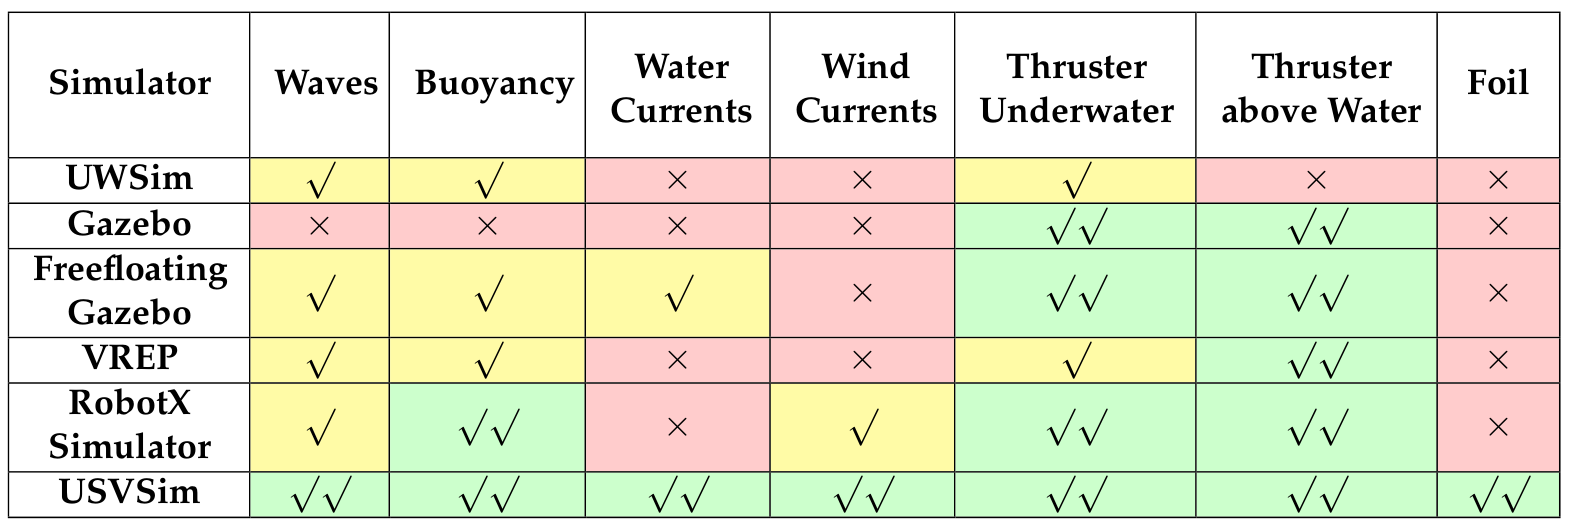
\includegraphics[width=14cm]{simComparison.png}
	\caption[Schematic Simulators Comparison]{Schematic recap of simulation comparison taken from \cite{usvsim}. $\times$ stands for no implemented feature; ~ $\surd\,$  for a feature that is a discrete representation of the real one; ~ $\surd\surd\,$ for a good representation of the real one. More details on how each feature is evaluated are available in the original paper.}
	\label{fig:simComparison}
\end{figure}


\section{Simulating the Firm Grasp Constrain}
\label{sec:firmGrasp}
Due to the limitation of the used simulator (explained in section \ref{sec:simulators}), some tricks have to be made. Without dynamics, simulate correctly the grasp of the peg is impossible. The simulator permits to fake the grasping with an \textit{object picker} sensor: when an object is sufficiently near to the point where this sensor is, it becomes \enquote{grasped} and it will rigidly move with the whole robot. The problem here is that we have two robots that must take the tool, so the object can't rigidly move with both, but only with the first who catch it. Furthermore, external forces applied to an object (grasped or not) can't be detected with the force-torque sensor, because, as it is implemented, it only detects forces acting on a vehicle part.\\
To solve this, a peg is modelled as additional fixed joint for each robot. In this way, each peg is rigidly attached to its own robot. Now, the problem is how to maintain the two pegs perfectly coincident during the whole mission. This is needed because the control architecture assumes a \textit{firm grasping}. This means that the end-effector does not move respect to the peg, and, consequently, the end-effectors of the robots do not move respect themselves.\\
In the simulation, collisions between the \enquote{pegs} and the hole cause them to drive apart. This is because collisions are propagated to the robots with a formula which use Jacobian (detailed in section \ref{sec:forceConsideration}). Jacobian derives from approximation of non-linear relationship, so results are not perfect. So, during the transportation, but especially during the collision propagation in the insertion phase, the two pegs distance themselves a bit. So, the control point for one robot is in a different position of what it expect, that will cause even more diverging behaviour.\\
In real scenario, firm grasp act like a \enquote{glue}: if the end effector tends to go away from the grasping point, friction acts to maintain it to the contact point. This is true for very small errors; if the cooperation performance is bad, the common tool falls down or something breaks.\\
In the simulation, to fake the firm grasp, an additional routine is implemented: it simply calculates the distance between the two peg, and generates robot velocities to zeroing this distance. It is important to note that this is an help that we would have also in real scenario, as explained before. The only difference is that, in real scenario, if the errors are too big the end-effector begins to slip, and it will never return to its original grasping point. In this case, it returns always to the initial point. \\
The velocity generates by this routine are not so big to hide bad cooperation; so the tests are suitable to evaluate the proposed architecture, and to simulate real situation.

\section{Force-Torque Propagation}
\label{sec:forceConsideration}
When a robot interacts with the environment, each contact generates forces on it. Mission about assembling objects can't be studied in a properly manner without some considerations about these forces. In a peg-in-hole Mission, collisions between the peg and the hole will be transferred through the whole kinematic chain until the floating base, causing disturbance to the whole robotic system. Thus, it is necessary to simulate these behaviours.\\ 

Let us define $\boldsymbol{f} \in \mathbb{R}^3$ and $\boldsymbol{m} \in \mathbb{R}^3$ as:
\begin{equation}
\boldsymbol{f} = \begin{bmatrix}f_x \\ f_y \\ f_z\end{bmatrix} \qquad
\boldsymbol{m} = \begin{bmatrix}m_x \\ m_y \\ m_z\end{bmatrix}
\end{equation}
being the $\boldsymbol{f}$ and $\boldsymbol{m}$ the resultant forces and torques (projected on the tool frame $ \langle t \rangle $) of all the forces and torques acting on the tool. These disturbances generate joint velocities $ \dot{\boldsymbol{y}}_{\delta} \in \mathbb{R}^l$ [\cite{bookSiciliano}]:
\begin{equation}
	\label{eq:forTor}
	\dot{\boldsymbol{y}}_{\delta} \triangleq 
	\begin{bmatrix} \dot{\boldsymbol{q}}_{\delta} \\ \boldsymbol{v_1}_{\delta} \\ \boldsymbol{v_2}_{\delta} \end{bmatrix}
	= \begin{bmatrix} k_q \\ k_{v1} \\ k_{v2} \end{bmatrix} \, \begin{bmatrix}\;(^{lin}\boldsymbol{J}_t)^T \boldsymbol{f} + \;(^{ang}\boldsymbol{J}_t)^T \boldsymbol{m}\end{bmatrix} 
	\qquad 0 < k_q, k_{v1}, k_{v2} < 1 
\end{equation}
where $J_t$ is the Jacobian which express how Cartesian velocity $\dot{\boldsymbol{x}}_t$ of the tool are affected by the system velocity vector  $\dot{\boldsymbol{y}}$; $lin, ang$ superscripts refer to \textit{linear} (top three rows) and \textit{angular} (bottom three rows) parts of $J_t$; $\dot{\boldsymbol{q}}_{\delta}$ is the velocity vector for joints caused by the collisions; $\boldsymbol{v_1}_{\delta}$ and $\boldsymbol{v_2}_{\delta}$  are the linear velocity and angular velocity of vehicle caused by the collisions; $k_q, k_{v1}, k_{v2}$ are positive gains smaller than $1$, in general different from each other  because we are considering different types of velocities.\\


\section{Assumptions}
It is important to detail the assumptions made during the simulation. Some problems, that are necessary to be taken into account in a real environment, are not explored. This is necessary due to the difficulty of the particular scenario chosen. In this section, the more important assumptions are summarized.

\begin{itemize}
	\item Simulation is only kinematic. This implies, for example, that the commanded velocity to the vehicle and the arm are accomplished \textit{instantaneously} and \textit{perfectly}. Another implication is that the movements of arm and of the vehicle don't influence each other at all. The only \enquote{dynamic} implemented is caused by collision between the peg and the hole, which \enquote{transfer} the forces and torques acting on the peg along the whole arm (as described in \ref{sec:forceConsideration}).
	
	\item The initial configuration shows the peg already \textit{correctly} grasped by both robots. Also, the position of where the end effector have grasped the tool and the peg dimensions are known. This implies that relative position between each robot and peg's tip is \textit{perfectly} known. Such a initial configuration has been chosen because the grasping phase and problems arising during cooperative transportation have been explored in others already cited project like MARIS and ROBUST (e.g in the work \cite{IntroMaris2}) and they are also part of different studies of the on-going project TWINBOT.
	
	
	\item Pose (linear and angular displacement) of the two carrying robots and of the vision robot respect a common inertial frame (denoted as \textit{w} - \textit{world} in the whole thesis) is known. In real situation, the pose underwater is always an issue and it is never really precise. Good precision can be provided, for example, after some works in mapping the seafloor, which will provide a common reference point somewhere. Note that it is not important know the pose of the robot respect to a point above the water surface (that can be done thanks to information shared with surface vessels, for example as explored the WiMUST project [\cite{wimust}]). The important thing is to know relative pose of the robots to a common node, that can also be underwater. This is needed to make the vision robot share correctly the estimated hole's pose with the carrying robots.
	
	\item No real communication issues between the two carrying robot are taken into account. The presence of water puts important issues in real situation: \textit{full-duplex} communication (i.e. sharing data \textit{at the same time}) is impossible, and, in general, there is a lower bandwidth than in the air. Some experiments in simulated environment with different methods of underwater communication are detailed in \cite{IntroMaris2}.\\
	However, these issues are considered by the cooperative scheme (explained in section \ref{sec:coopScheme}); in fact it permits to exchange very few information between the two carrying agents.
	
	\item The two robots firmly grasp the peg. There is no sliding caused by robot movements. This point is detailed in section \ref{sec:firmGrasp}.
	
	\item During the insertion phase, the architecture resolve alignment errors \textit{only if} the peg is inside the hole. If the peg touches the external hole surface, no routines are implemented to deal with the problem of \textit{looking} for the hole on the surface.
	
	\item The sensor is positioned on the tip of the peg, and it provides forces and torques caused by contacts with the whole peg. This would obviously not possible in real applications. In real scenario the sensor is usually put on the wrist and provide forces respect to this point. However, we could project the force-torque sensor information on another frame, if we know the relative pose. This assumption is also necessary because the chosen simulator can give force-torque information only on the part where the sensor is positioned.\\
	Also, both robots have access to the sensor data, without uncertainties (except numerical errors due to how almost all physics engines compute collisions, that it is done with approximations to improve the performance).
	
	%todo altre? 
\end{itemize}

\noindent Others assumptions, more related to the vision part, are detailed in section \ref{sec:visioAssumption}.

\section{Control Loop}
\begin{figure}[H]
	\centering
	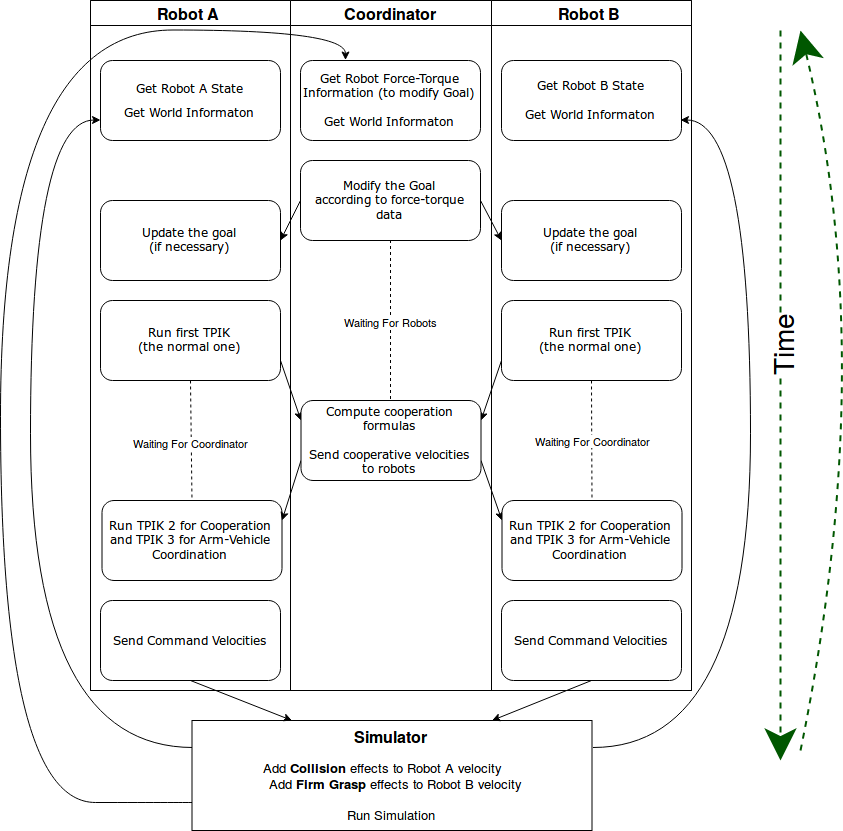
\includegraphics[width=12cm]{flowScheme.png}	
	\caption[Flow Scheme Control Loop]{A flow scheme showing the main step of a single control loop for the robots and for the coordinator. Blocks at the same horizontal level are executed at the same time. Arrows show connection between blocks of different nodes. Note here that the vision robot is not considered}
	\label{fig:flowScheme}
\end{figure}

This section is made to give a better idea on how the control architecture works.\\
The Vision Robot, which job is to estimate the hole pose, acts in a preliminary phase. It \textit{tracks} the hole, thanks to stereo-cameras, and it sends the estimated pose to the two carrying robots (and to the Coordinator). Due to its nature, no complicated control is implemented for this agent: when the pose is sent, we simply move it away from the hole with keyboard (like a ROV) to not interfere with the insertion mission. This part is described in Chapter \ref{chap:vision}.\\

The two carrying robots are completely autonomous: as soon they get the hole pose, they start, \textit{without user intervention}, the main mission. There are three nodes: the two Robots (\textit{A} and \textit{B}) and the Coordinator. The latter is not a real \textit{physical} agent: it is only a software routine. So, it can be physically inside one robot, let's say Robot A. In this way, communication issues (due to the underwater scenario) happen only between the two robots, and not among all the three nodes.\\
Initially, the Agent A, the Agent B and the Coordinator synchronize themselves, i.e. each one waits that the other two are ready. After this initialization phase, the normal routine starts, as can be seen in figure \ref{fig:flowScheme}, where the main instructions of the control loop are depicted.
\begin{itemize}
	\item At the beginning of the control loop, each node gets the updated simulation state, e.g. pose of the robots, pose of the tool, information from force-torque sensor, and so on.
	
	\item The Coordinator, which (as said previously and without loss of generality) is a software routine inside the Robot A, modifies the goal's linear position (as explained in \ref{sec:changeGoal}), if some forces are detected. If the goal is updated, the two Agents get this new information.
	
	\item In the third block's row, the Robots run the first TPIK procedure. Then, they send the necessary data to the Coordinator, which computes the cooperative velocities and sends them back to the robots. Finally, the two Agents run another two TPIK procedures, one for the cooperation and the other for the vehicle-arm coordination. This routines are described in Section \ref{sec:armVehScheme} and Section \ref{sec:coopScheme}. In all the TPIK procedure, the force-torque objective (Section \ref{sec:forceTask}) is used.
	
	\item At the end, the two Agents send the outputs (i.e., the system velocity vectors) to the simulation.
	
	\item Before sending the velocities to the \enquote{real} simulation, some disturbances must be added to the commanded system velocity vectors. For the Robot A, this means adding effects of collisions between the peg and the hole (Section \ref{sec:forceConsideration}). Instead, for the Robot B, effects of the firm grasp constrain are added (Section \ref{sec:firmGrasp}).
	
	\item After the simulation performs a step, the routine starts again.
	
\end{itemize}
\vspace{20px}
It can be noticed that the two added physical interactions (collisions and firm grasping constrain) are added only for one robot (A and B, respectively) and not for both.\\
This is done to not add simulation errors that can occur, and that would not happen in real scenario. For example, in real situation there are not two coincident pegs (as in this simulation) and so they can't really distinguish themselves. Putting the firm grasp constrain only on one robot helps to reduce disturbances that in real scenario are not present. Also, it is sufficient to fake a real firm grasping.\\
About the collisions, they affect, \textit{directly}, only the first agent. In truth, they also affect the other one, \textit{indirectly}, because the latter is \textit{dragged} by the firm grasp constrain. So, practically, collisions affect the behaviours of both agents.\\
It is important to notice that these physical interactions do not hide control problems: if the control is setted badly, the whole mission fails (e.g. the two peg diverge and/or compenetrate visibly with the hole).\\
%%%%
Another thing to notice is that, when the force-torque objective (Section \ref{sec:forceTask}) is used, both Robots need the sensor data. Being the force-torque sensor only on Robot A, this means that additional communication between Robot A and Robot B is needed. As known, underwater transmission is difficult and slow, and the general amount of the exchanged data should be keep as small as possible (from this problem it derives the used coordination policy).\\ 
An alternative can be to use another sensor on the Robot B. The problem following this direction could be that different sensors give not exactly same data. So, the two robots run each TPIK with different information. This problem is not explored here.\\
Another solution can be simply to avoid using this objective: it would decrease the performance of the mission (as we will see later) but results are good anyway.

\section{Results}
\begin{figure}[H]
	\centering
	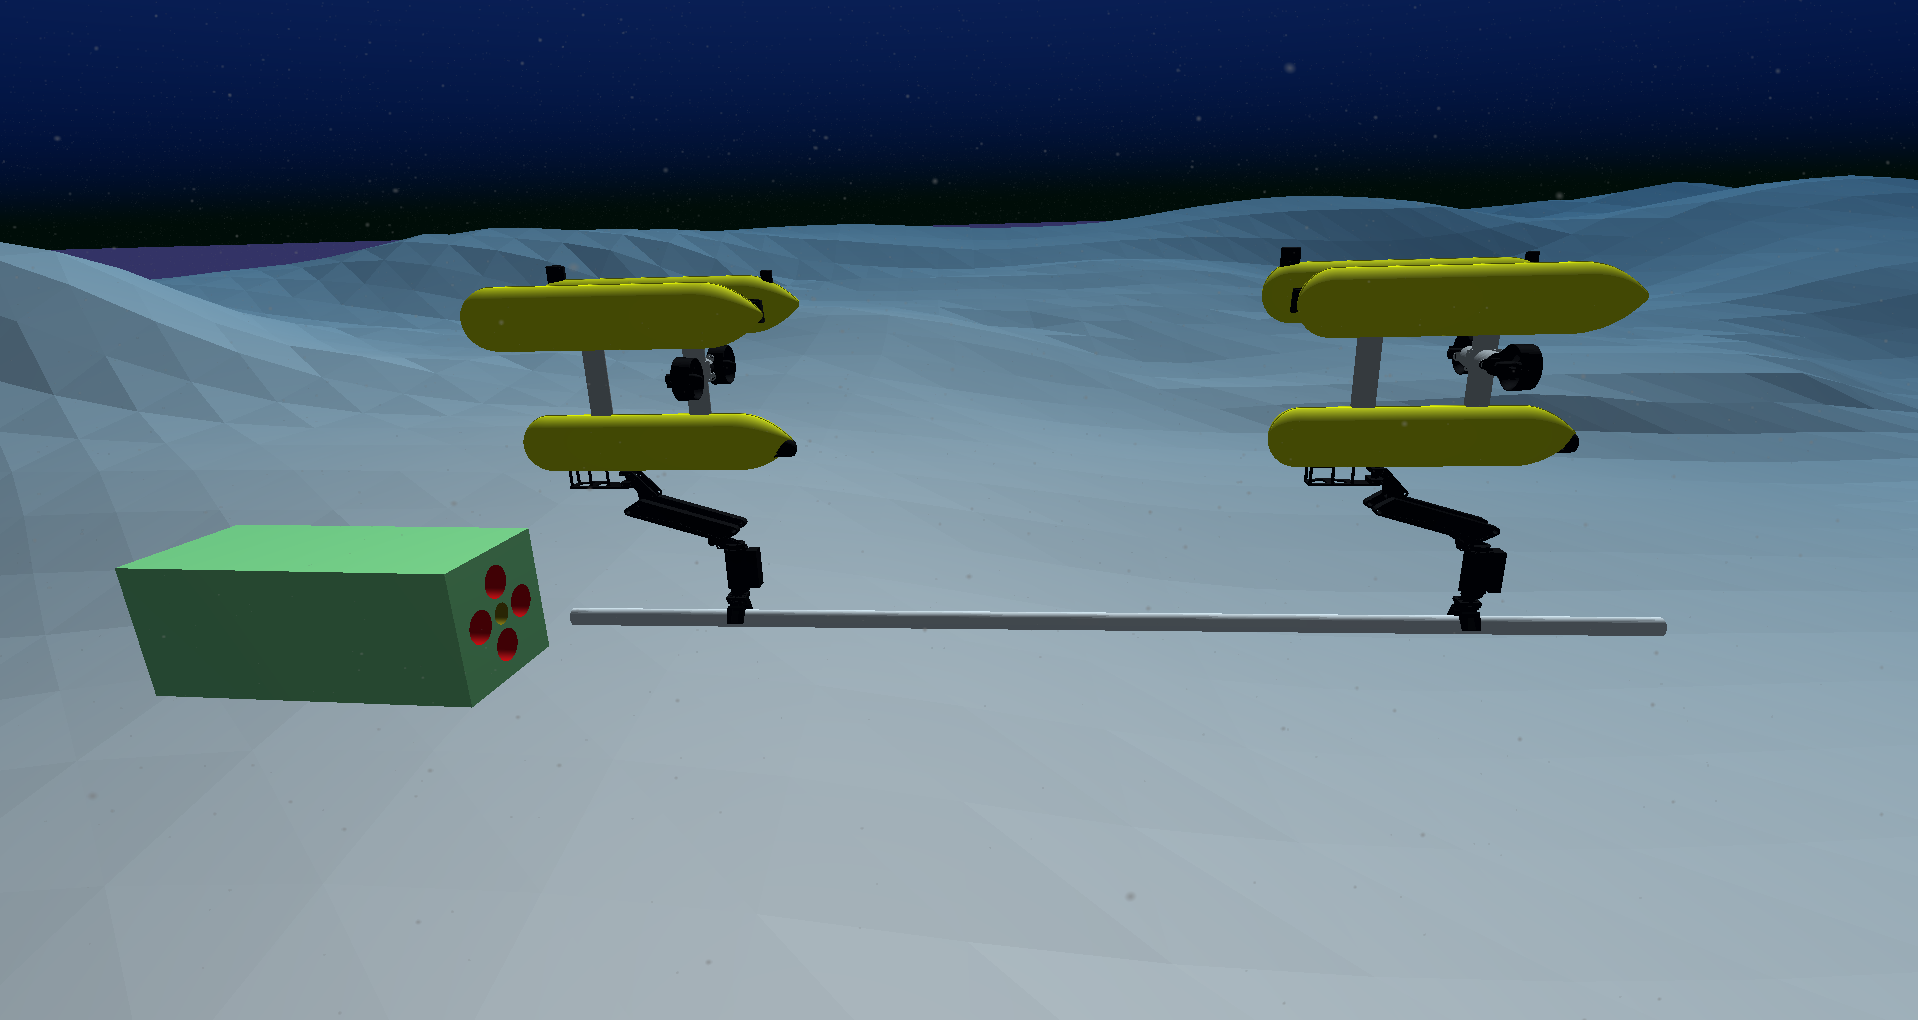
\includegraphics[width=10cm]{scenario_onlyTwin.png}
	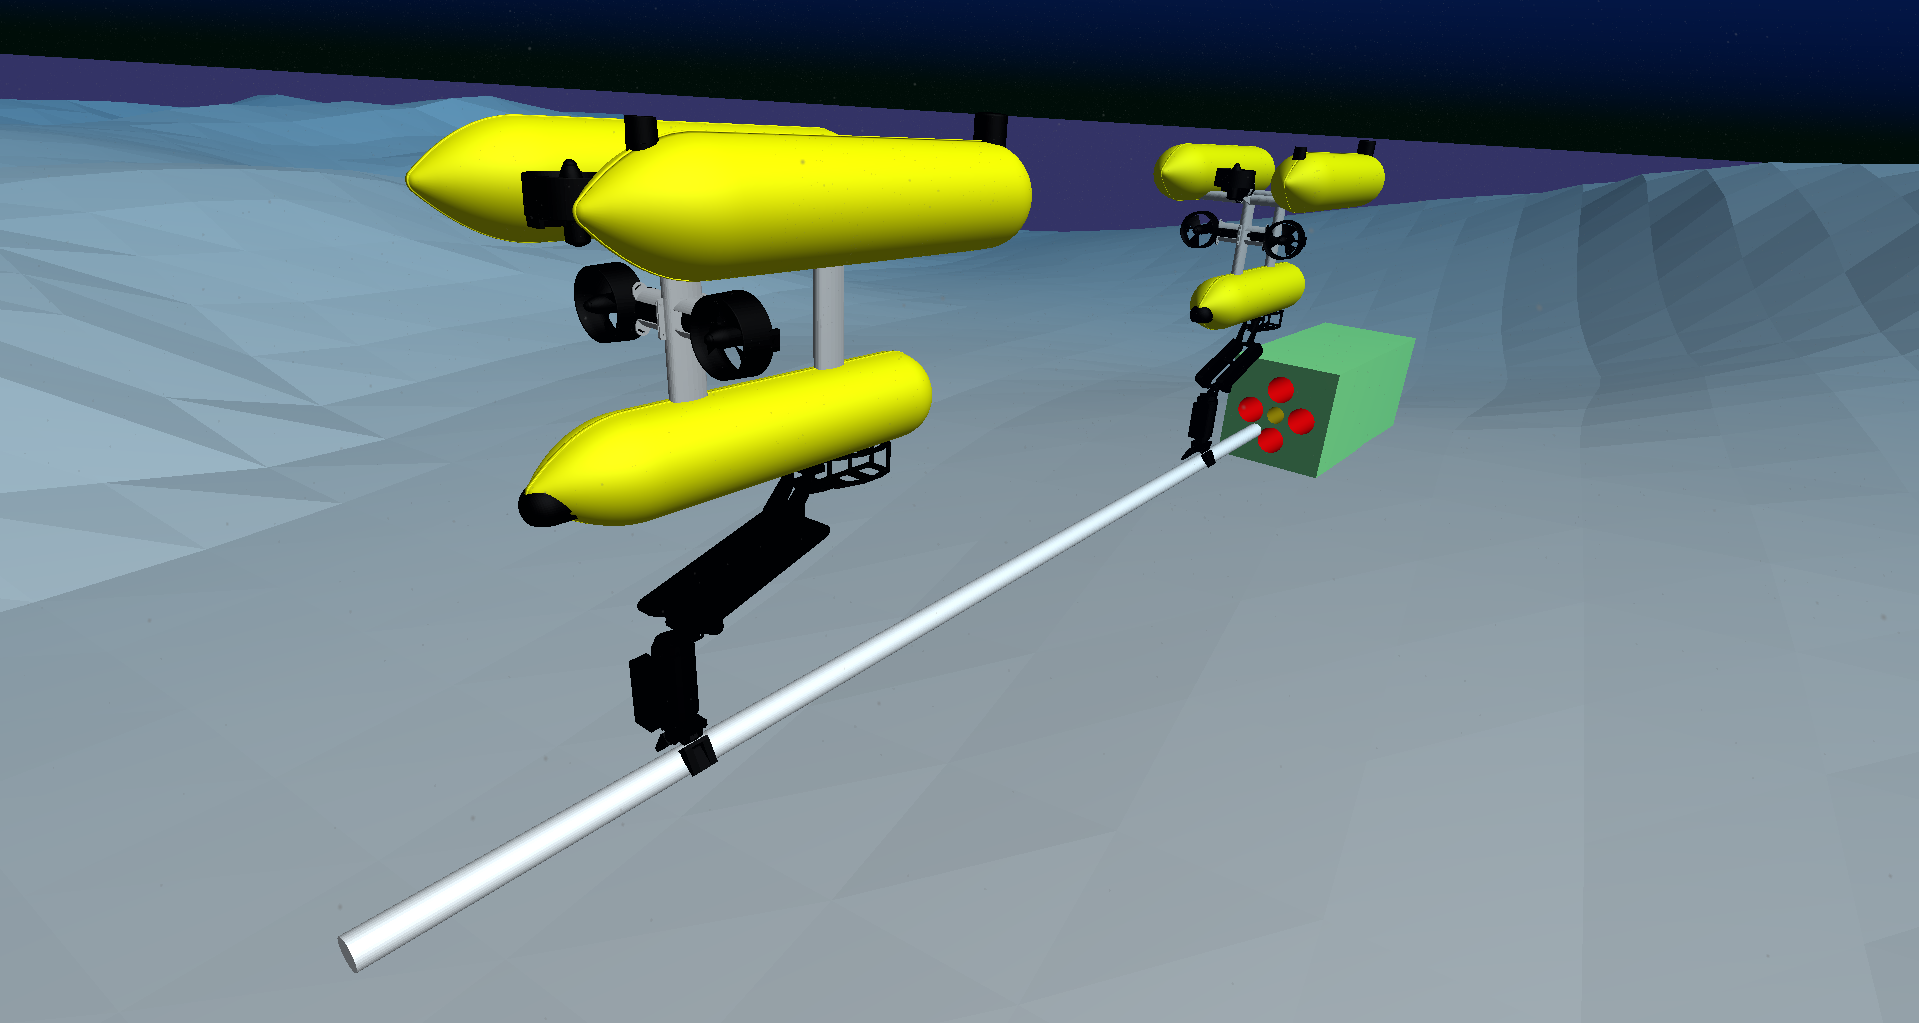
\includegraphics[width=10cm]{scenario_onlyTwin2.png}
	
	\caption[Scenario for test without the vision part]{Two differents angle view of the initial scenario for the results presented in this section. The pose estimation with vision is here neglected and the goal frame considered known without any errors.}
	\label{fig:onlyTwin_uwsim}
\end{figure}

{\LARGE TODO}